\documentclass[conference,a4paper]{IEEEtran}
% IEEE Xplore accepts PDF 1.4 to 1.7; pin 1.5 when building with pdfLaTeX (IEEE's reference toolchain).
\ifdefined\pdfminorversion\pdfminorversion=5\fi
% Camera-ready only: uncomment the next two lines and \IEEEpubidadjcol after \maketitle,
% and replace the placeholder with the copyright line supplied by the conference.
% \IEEEoverridecommandlockouts
% \IEEEpubid{\makebox[\columnwidth]{979-8-XXXX-XXXX-X/26/\$31.00~\copyright2026 IEEE\hfill}\hspace{\columnsep}\makebox[\columnwidth]{\hfill}}
\usepackage{cite}
\usepackage{amsmath}
\usepackage[T1]{fontenc}
\usepackage{newtxtext,newtxmath}
\usepackage{graphicx}
\usepackage{booktabs}
\usepackage{tabularx}
\usepackage{array}
\usepackage{microtype}
\usepackage{xcolor}
\usepackage{url}

% Public repository with the code, saved results, and paper sources.
\newcommand{\repourl}{\url{https://github.com/Research-maniacs/stockout-aware-demand-forecasting}}

\newcommand{\todo}[1]{\textcolor{red}{\textbf{TODO: #1}}}
\newcommand{\Dproxy}{D^{\mathrm{proxy}}}
\newcommand{\Sr}{S_{\mathrm{rec}}}

\begin{document}

\title{Stockout-Aware Demand Forecasting and Newsvendor Ordering on FreshRetailNet-50K}

% All authors share this affiliation; long names are split so four blocks fit in one row.
\newcommand{\srmaffiliation}{\textit{Dept. of Data Science and}\\
\textit{Business Systems}\\
\textit{SRM Institute of Science}\\
\textit{and Technology}\\
Chennai, Tamil Nadu, India}

\author{\IEEEauthorblockN{Akshara Kumari}
\IEEEauthorblockA{\srmaffiliation\\
{\small aksharakumari1208@gmail.com}}
\and
\IEEEauthorblockN{Aman Koley}
\IEEEauthorblockA{\srmaffiliation\\
{\small amankoley31530@gmail.com}}
\and
\IEEEauthorblockN{Shivam Singh}
\IEEEauthorblockA{\srmaffiliation\\
{\small shekhawat419shivam@gmail.com}}
\and
\IEEEauthorblockN{G. Premalatha}
\IEEEauthorblockA{\srmaffiliation\\
{\small premalag@srmist.edu.in}}}

\maketitle
% \IEEEpubidadjcol

\begin{abstract}
Recorded sales understate demand whenever a product sells out, so forecasts and orders fitted to sales inherit the stocking policy. We study demand forecasting and newsvendor ordering on FreshRetailNet-50K, a fresh-retail panel with hourly stockout flags. Days without a flagged stockout give an exact, though selected, proxy for demand. We censor these days with three simulated stockout mechanisms and score every forecast and order against the same uncensored outcomes, so models trained on differently censored histories are compared on identical rows. Earlier evaluations on this dataset score demand recovery and forecast accuracy, or profit measured on censored sales; we score ordering cost against an uncensored proxy and measure transfer between censoring mechanisms. In a 5,000-series run locked before the final week was scored, we compare nine ordering policies under three cost ratios; none wins under every ratio. When a shortage costs three times as much as a leftover unit, LightGBM demand quantiles with pooled conformal calibration are the cheapest full-sample policy in all nine train/test cells; when leftovers cost more, a raw-sales LightGBM with residual quantiles is cheapest in all nine. Training on a different mechanism raises the calibrated policy's mean cost by at most 0.0472 normalized units (95\% cluster-bootstrap interval 0.0391--0.0554), the smallest worst case among the policies that read the evaluation history. For real censored days, where demand is unobserved, we report only a lower bound on misses of the 90\% quantile forecast.
\end{abstract}

\begin{IEEEkeywords}
censored demand, stockouts, demand forecasting, quantile regression, conformal calibration, newsvendor, fresh retail
\end{IEEEkeywords}

\section{Introduction}
\label{sec:introduction}

Retailers record sales, not demand. When a product sells out, the record stops at the stock that was available and the unmet part of demand leaves no trace. A model fitted to such records learns the stocking policy along with customer behavior, and its errors carry into the next order. Fresh retail makes the cost immediate: tomorrow's order trades lost sales against perishable surplus, and a forecast that tracks recorded sales closely can still lead to a poor order if its history was censored~\cite{nahmias1994demand,huh2011adaptive}. For the same reason, a lower forecast error does not by itself show that one ordering policy is better than another. The comparison has to use the same outcome, the same cost ratio, and the same scored rows.

FreshRetailNet-50K~\cite{wang2025freshretailnet,dingdong2025datasetcard} makes this problem measurable because it records an hourly stock-status flag next to hourly sales. We use the flags in a narrow way. A series-day with no flagged stockout between 06:00 and 21:59 is a \emph{donor day}, and its recorded sales over that window serve as an exact proxy for demand, provided the flags are correct. Donor days are not a random sample: well-stocked and slow-moving items qualify more often, and the proxy says nothing about demand on days that were actually censored. Within that limit, donor days support a controlled experiment. Three simulated stockout mechanisms censor the histories of eligible donor days in different ways. Features and forecasts are rebuilt from each censored history, and every forecast is scored against the same uncensored proxy, so a model trained under one mechanism can be evaluated under another on identical target rows.

The evidence comes from three saved executions of one notebook pipeline (Fig.~\ref{fig:lineage}). Two standalone runs cover the development phases on a stratified 5,000-series sample (run~S) and on all 50,000 series (run~P). A third, end-to-end run (run~E) repeats the development phases on its own 5,000-series sample and continues through deep-learning baselines, a censored-inventory baseline, conformal calibration, ordering, a protocol lock, and a single evaluation of the final week. We keep the three runs apart. Runs~S and~E report identical tuning errors, yet they are different executions with different output files, and only run~E feeds the final evaluation.

Our contributions are an evaluation design and the evidence it produces, rather than a new forecasting architecture:
\begin{itemize}
\item a matched donor-proxy protocol that scores forecasts and orders trained on differently censored histories against identical outcomes, with the evaluation protocol locked before any final-week outcome was read;
\item a comparison of nine ordering policies under three cost ratios that reports the scored population and row count of every policy, including a separate panel for the neural policies, which cover only a declared subset of series;
\item the pre-specified paired contrasts and mechanism-transfer gaps with cluster-bootstrap intervals, and a lower bound on q90 misses for real censored histories, where no demand label exists.
\end{itemize}
The code, saved run outputs, and paper sources are available at \repourl.

\begin{figure}[t]
\centering
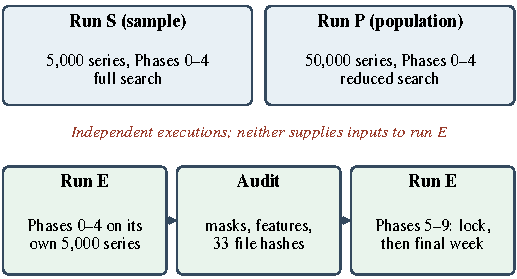
\includegraphics[width=\columnwidth]{figures/run_lineage.pdf}
\caption{The three saved executions. Only run~E's own Phase~0--4 stage feeds its prerequisite audit and the locked final evaluation; runs~S and~P are independent development evidence.}
\label{fig:lineage}
\end{figure}

\subsection{Related work}
\label{sec:related}

Estimating demand from sales truncated by stockouts is a long-standing inventory problem. Parametric methods fit a demand distribution to censored observations~\cite{nahmias1994demand}, and nonparametric policies learn order levels from censored sales with the Kaplan--Meier product-limit estimator~\cite{kaplan1958nonparametric,huh2011adaptive}; our Kaplan--Meier baseline follows the second idea with pooled support rules. Feature-based newsvendor methods learn an order directly from covariates~\cite{ban2019bignewsvendor}. Under linear shortage and surplus costs, the optimal order is a quantile of the demand distribution at the critical fractile, which ties ordering to quantile regression and its pinball loss~\cite{koenker1978regression}.

Our forecasters are gradient-boosted trees~\cite{ke2017lightgbm}, TimesNet~\cite{wu2023timesnet} for recovering masked hours, and the Temporal Fusion Transformer (TFT)~\cite{lim2021tft} for next-day forecasts. Calibration applies pooled split-conformal corrections in the spirit of conformalized quantile regression~\cite{romano2019cqr}, a sequential variant that updates its target miss rate as in adaptive conformal inference~\cite{gibbs2021adaptive}, and monotone rearrangement to remove quantile crossing~\cite{chernozhukov2010quantile}. The coverage guarantees of these methods rest on exchangeability or on explicit assumptions about how the data change; real stockout-censored days meet neither, so we measure coverage only where the donor proxy exists. Intervals come from a percentile cluster bootstrap~\cite{efron1979bootstrap}. The dataset report~\cite{wang2025freshretailnet} introduces the stockout annotations and a two-stage recovery-then-forecast baseline, whose official code~\cite{dingdong2025baseline} we reproduced only in part (Section~\ref{sec:deepdev}).

\section{Data and Experimental Protocol}
\label{sec:data}

\subsection{Data and outcome}
\label{sec:outcome}

The local training file has 4,500,000 series-day rows and the evaluation file 350,000. A series is a (city, store, product) triple, and the training panel contains 50,000 series. The local training file holds 865 distinct product identifiers, the number given on the current dataset card~\cite{dingdong2025datasetcard}; the pinned dataset report states 863 SKUs~\cite{wang2025freshretailnet}. The card labels the release as version 1.0 under a CC BY 4.0 license. The upstream revision and download date of our copies were not recorded, so the SHA-256 hashes in the availability statement are the only identifiers of the files used.

The outcome is the sum of recorded hourly sales from 06:00 to 21:59, the window a next-day order has to cover, rather than the full-day \texttt{sale\_amount}. A series-day is a donor if its stock-status flags $s_{j,t,h}$ sum to zero over that window; flags outside the window do not matter:
\begin{equation}
\begin{aligned}
I^{\mathrm{donor}}_{j,t}&=\mathbf{1}\!\left\{\sum_{h=6}^{21}s_{j,t,h}=0\right\},\\
\Dproxy_{j,t}&=\sum_{h=6}^{21}y^{\mathrm{sale}}_{j,t,h}
\quad \text{if } I^{\mathrm{donor}}_{j,t}=1.
\end{aligned}
\label{eq:donor}
\end{equation}
On a donor day the recorded window sales equal demand in the window, as long as the flags are correct. The donor set is shaped by the stocking process, however, since low-demand or generously stocked items qualify more often, and results on donors need not hold on censored days. In run~S, fit-period donor days had a pre-day two-week mean of recorded sales 0.91 times that of the other days and fell less often on promotion days (0.35 against 0.39). Real final-week rows with a flagged stockout have no demand label. We never score them for forecast error or order cost; Section~\ref{sec:real} treats them separately.

\subsection{Pipeline and chronological protocol}
\label{sec:protocol}

The pipeline has ten phases: the data contract and sampling (Phase~0), audit and past-only features (1), simulated censoring (2), conventional baselines (3), LightGBM demand quantiles (4), TimesNet and TFT (5), Kaplan--Meier (6), conformal calibration (7), ordering policies and the protocol lock (8), and final evaluation (9). Table~\ref{tab:split} gives the fixed chronological split. Sampling tiers and the initial simulator rules use fit-period data only, hyperparameters are chosen on the tuning window, and the calibration window is used for calibration alone. The 5,000-series samples are stratified by first-level category, sales tier, and stockout-rate tier.

\begin{table}[t]
\centering\footnotesize
\caption{Chronological Split Shared by All Runs}
\label{tab:split}
\begin{tabularx}{\columnwidth}{@{}llc>{\raggedright\arraybackslash}X@{}}
\toprule
Role & Days & Dates & Use \\
\midrule
Model fit & 1--60 & 2024-03-28 to 2024-05-26 & model fitting \\
Tuning & 61--75 & 2024-05-27 to 2024-06-10 & model selection \\
Calibration & 76--90 & 2024-06-11 to 2024-06-25 & calibration only \\
Final & 91--97 & 2024-06-26 to 2024-07-02 & locked evaluation \\
\bottomrule
\end{tabularx}

\end{table}

Features for a target date use only information available before that date. Target-day stockout flags, sales, weather, and promotion values are excluded because they are unknown when the order is placed, and lag and rolling features are shifted by at least one day. The prerequisite audit randomizes every target-day field and confirms that the target-day features do not change. Up to Phase~4, the evaluation file was read for its schema, identifiers, and dates only. Run~E wrote its protocol lock in Phase~8, before any final-week outcome was scored, and the final week has been used once, for the locked evaluation reported here. For each mechanism comparison the target donor keys and dates are identical and only the simulated history differs.

\subsection{Simulated censoring mechanisms}
\label{sec:mechanisms}

Each mechanism replaces the visible history of eligible donor days, those with enough past data, by a simulated censored history; real censored days keep their recorded values. The opening stock of series $j$ on day $t$ under mechanism $m$ is
\begin{equation}
Q^{(m)}_{j,t}=\max\!\left\{\mu^{\mathrm{past}}_{j,t}\,k^{(m)}_{j,t}\exp(\sigma_m z_{j,t}),\;q_{\mathrm{floor}}\right\},
\label{eq:simstock}
\end{equation}
where $\mu^{\mathrm{past}}_{j,t}$ is the mean recorded window sales over the preceding two weeks, $k^{(m)}_{j,t}$ a stock multiplier fitted on fit-period stockout patterns, $z_{j,t}$ a seeded standard normal draw that all mechanisms share, and $q_{\mathrm{floor}}$ a small floor. Visible hourly sales are the lesser of proxy sales and remaining stock. Mechanism~A (ordinary depletion) may add one refill of half the opening stock one to three hours after the first simulated stockout, with a probability estimated from real within-day recoveries. Mechanism~B (promotion-sensitive) follows A but multiplies the stock factor by 0.6 on days that were promotion days in the record, so those days deplete earlier; the promotion flag drives the simulator and is not a forecasting feature. Mechanism~C (sustained scarcity) halves A's multiplier, uses a fixed noise scale, and never refills (Fig.~\ref{fig:mechanisms}). Features are recomputed on every simulated history.

\begin{figure}[t]
\centering
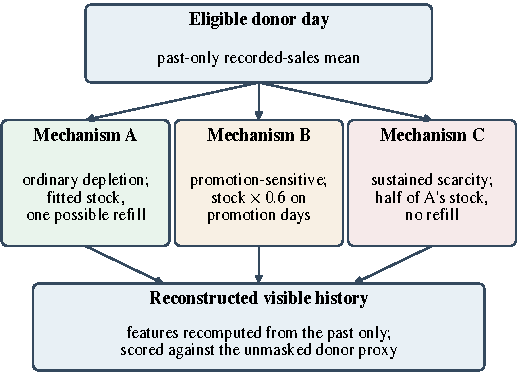
\includegraphics[width=\columnwidth]{figures/mechanism_paths.pdf}
\caption{The three censoring mechanisms act on eligible donor days. Each produces its own visible history, from which past-only features and forecasts are rebuilt; real censored days keep their recorded values.}
\label{fig:mechanisms}
\end{figure}

Within a transfer cell, defined by a training mechanism and an evaluation history, every forecast is scored against the same proxy outcome, so cost differences are paired. Across mechanisms, the masking rate and the distribution of reconstructed features change by design: B probes promotion-linked depletion and C persistent shortage. None of the mechanisms estimates how the retailer would behave under a real change of stocking policy.

\subsection{Models, calibration, and ordering}
\label{sec:models}

The conventional baselines are a seasonal-naive rule and LightGBM~\cite{ke2017lightgbm} point and quantile models trained on visible sales. The demand-quantile family trains LightGBM quantile models on donor-proxy targets at
\[
\tau\in\{0.25,0.50,0.75,0.90\},
\]
with one set per mechanism. On a declared deep subset of series, TimesNet recovers artificially hidden hours and TFT forecasts the next day either from the visible history (direct) or from the TimesNet-recovered history. The Kaplan--Meier policy estimates an order percentile from censored sales within pools that fall back from category by sales tier to category, management group, and a global pool when support is too small. Pooled conformal calibration shifts each quantile by a residual quantile computed on calibration-window donors in the same pool hierarchy, with a minimum pool size of 200, and then sorts the corrected quantiles of each row. The adaptive variant updates its target miss rate after each donor day, as in adaptive conformal inference~\cite{gibbs2021adaptive}, and serves as a sensitivity analysis. Point forecasters (seasonal naive, raw-sales LightGBM, and TFT) become quantile forecasts by adding the pooled quantile of their calibration residuals.

With a cost $c_u$ per unit short and $c_o$ per unit left over, the newsvendor order is the $\beta=c_u/(c_u+c_o)$ quantile of the forecast distribution. The cost of a row is
\begin{equation}
\begin{aligned}
C(Q,\Dproxy)={}&c_o\max(Q-\Dproxy,0)\\
&+c_u\max(\Dproxy-Q,0),
\end{aligned}
\label{eq:cost}
\end{equation}
evaluated against the unmasked donor proxy under a one-day shelf life. The locked settings are $(c_u,c_o,\beta)=(1,3,0.25)$, $(1,1,0.50)$, and $(3,1,0.75)$, which we call excess stock more costly, equal costs, and shortage more costly. Costs are in normalized sales units.

\subsection{Metrics}
\label{sec:metrics}

For a scoring population $\mathcal I$ of donor rows, we report the weighted absolute percentage error of the q50 forecast, the empirical coverage of $q_\tau$, and the pinball loss~\cite{koenker1978regression}:
\begin{align}
\mathrm{WAPE}&=\frac{\sum_{i\in\mathcal I}|\Dproxy_i-\widehat D_i|}{\sum_{i\in\mathcal I}\Dproxy_i}, \\
\widehat C_\tau&=\frac{1}{|\mathcal I|}\sum_{i\in\mathcal I}\mathbf{1}\{\Dproxy_i\le q_{\tau,i}\}, \\
\widehat P_\tau&=\frac{1}{|\mathcal I|}\sum_{i\in\mathcal I}
(\Dproxy_i-q_{\tau,i})(\tau-\mathbf{1}\{\Dproxy_i<q_{\tau,i}\}).
\label{eq:forecastmetrics}
\end{align}
The development files store WAPE as a ratio; the final forecast file stores it as a percentage. Coverage on calibration rows is only a diagnostic, because the same rows set the correction. On donor rows, forecast error, coverage, pinball loss, and order cost answer different questions, and we do not rank methods across them.

For a real final-week row, let $\Sr$ be the recorded window sales and $U_{90}$ the q90 forecast. Demand on a censored row is at least $\Sr$, so every row with $\Sr>U_{90}$ is a certain miss, whereas a row with $\Sr\le U_{90}$ may still hide one. The definite-miss rate
\begin{equation}
L_{\mathrm{miss}}=\frac{1}{n}\sum_{i=1}^{n}\mathbf{1}\{S_{\mathrm{rec},i}>U_{90,i}\}
\label{eq:miss}
\end{equation}
is therefore a lower bound on the real q90 miss rate. It is neither a coverage estimate nor an estimate of censored demand.

\section{Development Runs and Reproducibility}
\label{sec:scale}

Table~\ref{tab:scale} compares the two development runs. Run~S searched hyperparameters fully on 5,000 series; run~P used a reduced search on all 50,000 series. The overall donor share is almost the same (0.5580 and 0.5573), so the stratified sample preserves donor availability. Run~P has a lower q50 tuning WAPE for all three mechanisms and a longer runtime, but the runs differ in search mode as well as size, so neither difference can be attributed to scale and the runtimes are not a scaling benchmark. Fit-period donor days outnumber training rows because the first week of history only feeds lag features.

\begin{table}[t]
\centering\footnotesize
\caption{Development Runs, Phases~0--4 (Tuning Window; WAPE as a Ratio)}
\label{tab:scale}
\begin{tabular}{@{}lrr@{}}
\toprule
Measure & Run S & Run P \\
\midrule
Selected series & 5,000 & 50,000 \\
Selected series-days & 450,000 & 4,500,000 \\
Hyperparameter search & full & reduced \\
Fit donor days & 163,250 & 1,630,675 \\
Tuning donor days & 45,097 & 450,872 \\
Calibration donor days & 42,773 & 426,447 \\
Overall donor share & 0.5580 & 0.5573 \\
Training rows per mechanism & 144,078 & 1,440,065 \\
q50 tuning WAPE, A & 0.3334 & 0.3124 \\
q50 tuning WAPE, B & 0.3361 & 0.3144 \\
q50 tuning WAPE, C & 0.3358 & 0.3161 \\
Runtime (s) & 1,194.9 & 4,210.4 \\
Peak memory (GB) & 1.292 & 6.110 \\
\bottomrule
\end{tabular}

\end{table}

The simulator summaries agree between the two runs to within 0.001. The masked share, the fraction of eligible donor days with at least one simulated stockout hour in the window, is 0.460, 0.566, and 0.832 for A, B, and C in run~S (0.459, 0.567, and 0.832 in run~P), and the share of proxy sales left visible after simulation is 0.803, 0.718, and 0.474 (0.804, 0.717, and 0.474). The sample is therefore representative for these summaries; this does not show that the joint feature distribution, or any downstream metric, is the same at both scales.

Run~E did not reuse run~S. It executed its own Phase~0--4 stage, with the full hyperparameter search, in the same kernel as its later phases. Its fingerprints of the selected series, the chronological split, and the three simulator masks equal those of run~S, and so do its donor counts and its q50 tuning WAPEs at full stored precision (0.333440, 0.336140, and 0.335759 for A, B, and C). This is consistent with a deterministic pipeline applied to the same data, seed, and sampling rule. The two runs still differ in timestamps, pandas version (3.0.2 in run~S, 2.3.3 in run~E), and file hashes, so we treat them as separate evidence. Within run~E, one Phase~0 check stayed open because it compares fingerprints with an earlier execution in the same output folder, and the first execution has none; the comparison with run~S above is the one it would have made. Before continuing, a prerequisite audit re-derived the simulator masks and feature matrices from the raw panel, required exact agreement, and verified the hashes of 33 predecessor files. Run~E's later phases ran in the reduced mode, which uses 200 bootstrap replicates. No run hashed the notebook source it executed, so the current notebook files cannot prove which code produced a given result.

\section{Run~E: Models, Calibration, and the Lock}
\label{sec:complete}

All results from here on come from run~E and its 5,000 series. Its prerequisite audit passed 10 checks. Besides reproducing the simulator masks and features, it confirmed that proxy labels exist only on donor days and match a recomputation, that the calibration and final-week days were unused so far, and that randomizing target-day fields leaves the target-day features unchanged.

\subsection{Deep models on a declared subset}
\label{sec:deepdev}

The deep models ran on CPU, with two logical CPUs, 8.42~GB of RAM, and four training epochs per model, on a declared subset of 600 series. TimesNet recovers artificially hidden donor hours, and across the three mechanisms it scored 290,397 hidden hours (Table~\ref{tab:deepdev}). TFT forecasts the next day's window total on matched tuning donor days, and its WAPE is lower when it reads the TimesNet-recovered history than when it reads the visible history. The two tasks differ in target, unit, and denominator, and neither WAPE is comparable with the Phase~4 q50 WAPE on the full sample. The final TFT routes reuse 6 trained models; the 24 frozen prediction pipelines combine the direct and recovered variants with the three training mechanisms and four evaluation histories (A, B, C, and the real history).

\begin{table}[t]
\centering\footnotesize
\caption{Phase~5 Development Metrics on the 600-Series Deep Subset (WAPE as a Ratio)}
\label{tab:deepdev}
\begin{tabular}{@{}lllrr@{}}
\toprule
Route & Mech. & Scored unit & $n$ & WAPE \\
\midrule
TimesNet recovery & A & hidden donor hours & 58,449 & 0.917 \\
TimesNet recovery & B & hidden donor hours & 82,225 & 0.919 \\
TimesNet recovery & C & hidden donor hours & 149,723 & 0.934 \\
\midrule
TFT direct & A & tuning donor days & 5,407 & 0.453 \\
TFT direct & B & tuning donor days & 5,407 & 0.451 \\
TFT direct & C & tuning donor days & 5,407 & 0.453 \\
TimesNet$\rightarrow$TFT & A & tuning donor days & 5,407 & 0.414 \\
TimesNet$\rightarrow$TFT & B & tuning donor days & 5,407 & 0.413 \\
TimesNet$\rightarrow$TFT & C & tuning donor days & 5,407 & 0.415 \\
\bottomrule
\end{tabular}

\end{table}

Our reproduction of the official baseline~\cite{dingdong2025baseline} is partial. The as-documented TimesNet run failed on a blocked network download and completed only after a recorded patch that reads the verified local Parquet files; the upstream TFT training finished, but its prediction step was not run. The task-aligned TimesNet and TFT implementations used in this paper passed their own stage checks.

\subsection{Kaplan--Meier baseline and calibration}

The Kaplan--Meier policy passed all 8 of its unit tests and built 207 pools, each with a recorded support count; its minimum support thresholds were chosen on tuning donors. If a pool cannot support the requested percentile, the order is left unestimated rather than filled in from another policy, so the policy can score fewer rows than the candidate set.

Calibration used 513,276 residuals from the calibration window, pooled over mechanisms and quantile levels. The fallback share, the fraction of calibration rows corrected from a pool coarser than category by sales tier, was 0.061. Some rows still had crossing quantiles after the correction, and sorting each row's corrected quantiles removed every crossing. Sorting guarantees ordered quantiles, not calibrated ones.

\subsection{Ordering policies and the protocol lock}

Nine policies turn forecasts into orders (Table~\ref{tab:policies}). All 10 hand-computed checks of the order and cost arithmetic passed. The Phase~8 lock then fixed the policy names, cost settings, model and calibration files, planned comparisons, and bootstrap settings before Phase~9 read any final-week outcome. The final week has been scored once under this lock, and any revised protocol applied to the same week would be exploratory.

\section{Locked Final-Week Evaluation}
\label{sec:final}

The final evaluation scores donor rows only. Each of the nine transfer cells, one per pair of training mechanism and evaluation history, holds the same 20,641 final donor series-dates, and the six full-sample policies other than Kaplan--Meier are scored on all of them. Kaplan--Meier scores only rows with an estimable order, between 6,012 and 20,641 per cell, with the fewest in the C-trained cells when shortage is more costly. The two neural policies score the 2,510 final donor rows of the deep subset, and no predictions are imputed for the remaining 4,400 series. Tables therefore state each policy's population and row count.

\subsection{Policy comparison}
\label{sec:policies}

Table~\ref{tab:policies} gives the mean costs of the A-trained models on the A history under the three cost settings. The best full-sample policy depends on the cost ratio. On the A history, the raw-sales LightGBM with residual quantiles has the lowest cost when excess stock is more costly and, narrowly, at equal costs (0.3868 against 0.3891 for pooled conformal); the pooled-conformal policy has the lowest cost when shortage is more costly. The B history gives the same ranking. On the C history the pooled-conformal policy is already the cheaper of the two at equal costs (0.4094 against 0.4411), so averaged over the three matched histories it is cheaper at equal costs (0.3984 against 0.4075), as in Tables~\ref{tab:contrasts} and~\ref{tab:ablations}; the paired interval of that average difference contains zero. The Kaplan--Meier percentile is the most expensive full-sample policy in each setting of the table. Within the deep subset, TFT on the TimesNet-recovered history costs less than direct TFT in every matched history and cost setting, a comparison internal to that subset.

\begin{table*}[t]
\centering\footnotesize
\caption{Mean Newsvendor Cost of Every Locked Policy for A-Trained Models on the A History (Lowest Cost per Panel and Setting in Bold)}
\label{tab:policies}
\begin{tabular}{@{}llrrrr@{}}
\toprule
 & & & \multicolumn{3}{c}{Mean cost} \\
\cmidrule(l){4-6}
Policy & Population & $n$ & $\beta=0.25$ & $\beta=0.50$ & $\beta=0.75$ \\
\midrule
\multicolumn{6}{@{}l}{\emph{(a) Full-sample exact-donor candidates}} \\
Seasonal naive + residual quantile & Full sample & 20,641 & 0.6759 & 0.4430 & 0.7853 \\
Raw-sales LightGBM + residual quantile & Full sample & 20,641 & \textbf{0.5448} & \textbf{0.3868} & 0.7366 \\
Raw-sales quantile LightGBM & Full sample & 20,641 & 0.5749 & 0.3999 & 0.7503 \\
Demand-quantile LightGBM (uncalibrated) & Full sample & 20,641 & 0.5816 & 0.3946 & 0.7152 \\
Demand-quantile LightGBM + pooled conformal & Full sample & 20,641 & 0.5766 & 0.3891 & \textbf{0.6831} \\
Kaplan--Meier order percentile & Full sample & 20,641 & 0.8404 & 0.6520 & 1.3878 \\
Demand-quantile + adaptive calibration (sensitivity) & Full sample & 20,641 & 0.5815 & 0.3932 & 0.6963 \\
\midrule
\multicolumn{6}{@{}l}{\emph{(b) Declared deep subset of 600 series (separate population)}} \\
TFT (direct) + residual quantile & Deep subset & 2,510 & 0.6892 & 0.4949 & 0.9483 \\
TimesNet$\rightarrow$TFT + residual quantile & Deep subset & 2,510 & \textbf{0.6586} & \textbf{0.4687} & \textbf{0.8759} \\
\bottomrule
\end{tabular}

\end{table*}

Table~\ref{tab:contrasts} reports the paired contrasts that the lock pre-specified for the pooled-conformal policy, pooled over the three matched histories. Calibration lowers cost relative to the uncalibrated demand quantiles in all three settings, and the pooled-conformal policy is cheaper than the seasonal-naive and Kaplan--Meier policies throughout. Against the raw-sales LightGBM with residual quantiles the sign depends on the cost ratio: the pooled-conformal policy costs more when excess stock is more costly, the equal-cost interval contains zero, and it costs less when shortage is more costly.

\begin{table*}[t]
\centering\footnotesize
\caption{Pre-Specified Paired Contrasts for the Pooled-Conformal Policy over the Three Matched Histories (Negative Values Favor Pooled Conformal)}
\label{tab:contrasts}
\begin{tabular}{@{}lllrrr@{}}
\toprule
Pooled conformal minus & Cost setting & Population & $n$ & Difference & 95\% percentile interval \\
\midrule
Uncalibrated demand quantile & Excess stock more costly & Matched full sample & 61,923 & $-0.0052$ & $[-0.0068, -0.0034]$ \\
Uncalibrated demand quantile & Equal costs & Matched full sample & 61,923 & $-0.0077$ & $[-0.0096, -0.0062]$ \\
Uncalibrated demand quantile & Shortage more costly & Matched full sample & 61,923 & $-0.0420$ & $[-0.0483, -0.0365]$ \\
\addlinespace
Raw-sales LightGBM + residual & Excess stock more costly & Matched full sample & 61,923 & $+0.0208$ & $[0.0016, 0.0432]$ \\
Raw-sales LightGBM + residual & Equal costs & Matched full sample & 61,923 & $-0.0091$ & $[-0.0204, 0.0052]$ \\
Raw-sales LightGBM + residual & Shortage more costly & Matched full sample & 61,923 & $-0.0790$ & $[-0.0946, -0.0615]$ \\
\addlinespace
Seasonal naive + residual & Excess stock more costly & Matched full sample & 61,923 & $-0.1213$ & $[-0.1465, -0.0876]$ \\
Seasonal naive + residual & Equal costs & Matched full sample & 61,923 & $-0.0694$ & $[-0.0872, -0.0439]$ \\
Seasonal naive + residual & Shortage more costly & Matched full sample & 61,923 & $-0.1376$ & $[-0.1723, -0.0902]$ \\
\addlinespace
Kaplan--Meier percentile & Excess stock more costly & KM-supported rows & 61,523 & $-0.4043$ & $[-0.4276, -0.3824]$ \\
Kaplan--Meier percentile & Equal costs & KM-supported rows & 58,183 & $-0.3223$ & $[-0.3429, -0.3046]$ \\
Kaplan--Meier percentile & Shortage more costly & KM-supported rows & 47,294 & $-0.7475$ & $[-0.8175, -0.6812]$ \\
\bottomrule
\end{tabular}

\end{table*}

\subsection{Service, surplus, and coverage}

Table~\ref{tab:scenarios} shows the pooled-conformal policy in each matched history. Moving from $\beta=0.25$ to $\beta=0.75$ raises the fill rate on the A history from 0.614 to 0.891 and the leftover share from 0.056 to 0.226. The critical fractile moves the order along the trade-off between service and surplus without removing it. Mean costs are not comparable across settings because the cost weights differ. The C history is the most expensive in every setting.

\begin{table}[t]
\centering\footnotesize
\caption{Pooled-Conformal Policy in the Matched Histories}
\label{tab:scenarios}
\begin{tabular}{@{}llrrrr@{}}
\toprule
History & Population & $n$ & Mean cost & Fill rate & Leftover \\
\midrule
\multicolumn{6}{@{}l}{\emph{Excess stock more costly ($\beta=0.25$)}} \\
A & Full sample & 20,641 & 0.5766 & 0.614 & 0.056 \\
B & Full sample & 20,641 & 0.5825 & 0.608 & 0.056 \\
C & Full sample & 20,641 & 0.5978 & 0.589 & 0.055 \\
\midrule
\multicolumn{6}{@{}l}{\emph{Equal costs ($\beta=0.50$)}} \\
A & Full sample & 20,641 & 0.3891 & 0.775 & 0.124 \\
B & Full sample & 20,641 & 0.3967 & 0.769 & 0.125 \\
C & Full sample & 20,641 & 0.4094 & 0.753 & 0.122 \\
\midrule
\multicolumn{6}{@{}l}{\emph{Shortage more costly ($\beta=0.75$)}} \\
A & Full sample & 20,641 & 0.6831 & 0.891 & 0.226 \\
B & Full sample & 20,641 & 0.6940 & 0.888 & 0.228 \\
C & Full sample & 20,641 & 0.7248 & 0.878 & 0.227 \\
\bottomrule
\end{tabular}

\end{table}

Pooled calibration also moves the empirical q90 coverage of the 20,641 matched final donor rows toward the nominal 0.90 in every history, from 0.798--0.828 to 0.879--0.887, and lowers the q90 pinball loss from 0.119--0.131 to 0.109--0.114. Coverage stays below nominal. It is measured on selected complete days after the calibration window, so it does not show that exchangeability holds for censored days or would survive a change of stocking policy.

\subsection{Mechanism transfer}
\label{sec:transfer}

Table~\ref{tab:transfer} fixes the pooled-conformal policy at $\beta=0.75$ and varies the history used for training and calibration. The transfer gap
\begin{equation}
\Delta_{m\to h}=\overline{C}_{m\to h}(\mathcal I)-\overline{C}_{m\to m}(\mathcal I)
\label{eq:transfer}
\end{equation}
compares the mean cost on an unseen evaluation history $h$ with the matched cost on the same rows $\mathcal I$. The largest gap arises for models trained on A and evaluated on C: 0.7303 against 0.6831, a gap of $+0.0472$. Training on B and evaluating on C also raises the cost. The C-trained models, in contrast, cost less on the A and B histories than on their own, consistent with the C history being the hardest to forecast from (Table~\ref{tab:scenarios}). A negative gap therefore signals an easier evaluation history rather than better transfer, and gaps combine a change of model with a change of difficulty.

\begin{table*}[t]
\centering\footnotesize
\caption{Transfer Gaps of the Pooled-Conformal Policy When Shortage Is More Costly}
\label{tab:transfer}
\begin{tabular}{@{}cclrrrrr@{}}
\toprule
Train & Test history & Population & $n$ & Matched & Unseen & Gap & 95\% percentile interval \\
\midrule
A & B & Full sample & 20,641 & 0.6831 & 0.6932 & $+0.0101$ & $[0.0076, 0.0128]$ \\
A & C & Full sample & 20,641 & 0.6831 & 0.7303 & $+0.0472$ & $[0.0391, 0.0554]$ \\
B & A & Full sample & 20,641 & 0.6940 & 0.6908 & $-0.0032$ & $[-0.0059, -0.0006]$ \\
B & C & Full sample & 20,641 & 0.6940 & 0.7306 & $+0.0365$ & $[0.0275, 0.0447]$ \\
C & A & Full sample & 20,641 & 0.7248 & 0.7120 & $-0.0128$ & $[-0.0219, -0.0050]$ \\
C & B & Full sample & 20,641 & 0.7248 & 0.7086 & $-0.0162$ & $[-0.0242, -0.0083]$ \\
\bottomrule
\end{tabular}

\end{table*}

All intervals are 95\% percentile intervals from 200 cluster-bootstrap replicates~\cite{efron1979bootstrap}. Each replicate resamples the 866 city--store clusters with replacement and keeps every row of a drawn cluster, and both sides of a contrast use the same draws. Dates are not resampled separately and no multiplicity adjustment is applied. With 200 replicates the tail percentiles are approximate, so we read the intervals as descriptive and make no claims of statistical significance.

\subsection{Robustness across cells, dates, and series}
\label{sec:robust}

The reversal with the cost ratio is not specific to the matched histories. Over all nine train/test cells, the raw-sales LightGBM with residual quantiles is the cheapest full-sample policy in every cell when excess stock is more costly, with the pooled-conformal policy 0.0007 to 0.0323 more expensive; when shortage is more costly, the pooled-conformal policy is the cheapest in every cell, 0.0441 to 0.1298 below the raw-sales policy. At equal costs the cells split: four go to each of the two policies and one to the uncalibrated demand quantiles. Over the three cost settings, the largest transfer gap of the pooled-conformal policy is $+0.0472$, the smallest worst case among the six policies whose forecasts read the evaluation history; the raw-sales quantile LightGBM reaches $+0.2258$. Kaplan--Meier orders do not read that history, so its gaps are zero by construction. Over the seven final dates, with 2,507 to 3,385 donor rows each, the C history is the most expensive on every date in all three cost settings, and the daily q90 coverage of the pooled-conformal models ranges from 0.839 to 0.907. Under-coverage concentrates in series with at most ten complete days in the fit period (q90 coverage 0.752 to 0.769 over 532 rows) and on promotion days (0.854 to 0.865). These breakdowns are descriptive outputs of the same locked run, not pre-specified comparisons, and carry no intervals.

\subsection{Real recorded histories}
\label{sec:real}

The q90 forecasts of the three pooled-conformal models were applied to the same 35,000 real final-week rows, 105,000 forecast rows in all, including rows with flagged stockouts. Table~\ref{tab:real} gives the definite-miss lower bound of \eqref{eq:miss}. A smaller bound can come from a higher forecast, so it does not by itself indicate better calibration. Across strata, the bound is highest for rows with 1--4 recorded stockout hours and lowest for 9--16 hours. Heavy censoring weakens the test: when a product sells out early, recorded sales can fall far below demand and seldom exceed the forecast even when demand does. Only the complete-day stratum has an exact proxy.

\begin{table}[t]
\centering\footnotesize\setlength{\tabcolsep}{4pt}
\caption{Definite-Miss Lower Bounds on Real Final-Week Rows, Overall (with 95\% Percentile Cluster-Bootstrap Intervals) and by Recorded Stockout Hours}
\label{tab:real}
\begin{tabular}{@{}llrrr@{}}
\toprule
Trained on & Population & Rows & Bound & 95\% interval \\
\midrule
A & Real history & 35,000 & 0.0895 & $[0.0852, 0.0942]$ \\
B & Real history & 35,000 & 0.0854 & $[0.0808, 0.0896]$ \\
C & Real history & 35,000 & 0.0724 & $[0.0684, 0.0766]$ \\
\bottomrule
\end{tabular}

\vspace{6pt}

\begin{tabular}{@{}lrrrr@{}}
\toprule
Recorded stockout hours & Rows & A & B & C \\
\midrule
0 (complete day) & 20,641 & 0.0730 & 0.0708 & 0.0579 \\
1--4 & 4,614 & 0.1797 & 0.1708 & 0.1465 \\
5--8 & 4,980 & 0.1283 & 0.1169 & 0.1044 \\
9--16 & 4,765 & 0.0334 & 0.0327 & 0.0298 \\
\bottomrule
\end{tabular}

\end{table}

\section{Discussion and Limitations}
\label{sec:discussion}

The ablations recorded in run~E (Table~\ref{tab:ablations}) are consistent with the locked comparisons. At equal costs over the matched histories, the pooled-conformal demand quantiles had a mean cost of 0.3984 against 0.4075 for the raw-sales point model with residual quantiles. Pooled calibration moved q90 coverage from 0.8121 to 0.8832 against a nominal 0.90. The adaptive variant cost 0.4039 against 0.3984 for static calibration, so its drift correction did not pay off in this week. A hypothetical two-day carry-over of unsold stock lowered the cost from 0.3984 to 0.2579, which shows how much the cost level depends on the one-day shelf-life assumption. Giving the model the target-day weather and promotion values, which are unknown when the order is placed, changed the q50 WAPE only from 33.48\% to 33.40\%. A reduced-lag ablation was not run, because fitting a new model after the final week had been scored would fall outside the lock.

\begin{table}[t]
\centering\scriptsize
\caption{Ablations Recorded in Run~E, as Pairs of Values in the Order Named (Mean Order Cost at Equal Costs Unless the Scope Says Otherwise)}
\label{tab:ablations}
\begin{tabularx}{\linewidth}{@{}>{\raggedright\arraybackslash}Xl>{\raggedright\arraybackslash}p{0.34\linewidth}@{}}
\toprule
Recorded diagnostic & Values & Scope \\
\midrule
Raw-sales vs.\ demand-quantile & 0.4075 / 0.3984 & Equal-cost matched cells \\
Uncalibrated vs.\ pooled q90 coverage & 0.8121 / 0.8832 & Final donor proxy; nominal 0.90 \\
Direct vs.\ recovered-history TFT & 0.4999 / 0.4690 & Equal-cost deep subset \\
Short vs.\ full lag set & Not available & Not run after the lock \\
Static vs.\ adaptive calibration & 0.3984 / 0.4039 & Equal-cost sensitivity \\
One-day vs.\ two-day inventory & 0.3984 / 0.2579 & Hypothetical carry-over \\
Contract vs.\ oracle-weather WAPE & 33.48\% / 33.40\% & Target-day oracle; not deployable \\
\bottomrule
\end{tabularx}

\end{table}

The main limitations are the following.
\begin{itemize}
\item \emph{Selected proxy.} Donor-day sales equal demand only on complete days, and which days are complete depends on demand and stocking. The proxy does not identify demand on censored days, and the real-history analysis gives only a lower bound.
\item \emph{Simulated mechanisms.} Mechanisms A, B, and C are specified simulations, not counterfactual inventory paths. The transfer results measure sensitivity to these constructed histories, not transport to another retailer or stocking policy.
\item \emph{Different populations.} The neural policies cover the 600-series subset, and Kaplan--Meier scores only estimable rows. A comparison of all policies on a common population would be a new analysis after the final week was exposed and would have to be labeled as such.
\item \emph{Cost model.} Rankings depend on the locked cost ratios and on the one-day shelf life.
\item \emph{Deep models.} The TFT and TimesNet routes were trained with a small CPU and epoch budget, and the official baseline was reproduced only in part.
\item \emph{Final-week exposure.} The final week was opened once under the Phase~8 lock. Any later protocol evaluated on it is exploratory. A future evaluation on all 50,000 series would contain the 5,000 series already scored and should report the remaining series separately.
\item \emph{Intervals.} The intervals come from only 200 bootstrap replicates, so their tails are approximate; dates are not resampled separately, and no multiplicity adjustment is made.
\item \emph{Provenance.} No run hashed the notebook source it executed, and the upstream dataset revision and download date are unknown; the local file hashes are the operative identifiers. All runs executed on Linux with Python 3.11.15, two logical CPUs, and 8.42~GB of RAM, run~E without a GPU. The released outputs omit large intermediate files, so Phase~5 cannot be resumed from them without regenerating Phases~0--4.
\end{itemize}

Every table and figure is generated by a script from the saved output files of the three runs, without retraining any model.

\section{Conclusion}
\label{sec:conclusion}

A matched donor-proxy design makes stockout-aware forecasting and ordering comparisons on FreshRetailNet-50K checkable: models trained on differently censored histories are scored against the same outcomes, under a protocol fixed before the final week was read. Within this design, the value of calibrated demand quantiles depends on the cost ratio. They gave the lowest cost when shortage was more costly, while a raw-sales point model with residual quantiles was cheaper when excess stock was more costly. Evaluating the calibrated policy on an unseen mechanism raised its cost by at most 0.0472 normalized units, and TimesNet-recovered histories lowered TFT order costs within the deep subset. These findings hold for donor days, the simulated mechanisms, and the locked cost settings. Testing them on censored demand itself, or on series outside the evaluated sample, requires a new protocol.

\section*{Code and Data Availability}
\label{sec:availability}

The code, the saved run outputs, and the paper sources are available at \repourl. The repository holds the notebooks, the saved run outputs used here, and the scripts that regenerate the tables and figures. Runs~S, P, and~E are stored under \path{results/phase0_4/demo5000/}, \path{results/phase0_4/full50k/}, and \path{results/phase0_9_5k/}; in run~E, \path{manifests/final_test_lock.json} holds the locked protocol and \path{phase9_evaluation/final_order_metrics.csv} the scored population and row count of every policy. The repository does not redistribute the dataset, which is available from Hugging Face~\cite{dingdong2025datasetcard} under its CC BY 4.0 license. The upstream revision and download date of our copies were not recorded, so the local files are identified by their SHA-256 hashes below. The last line is the SHA-256 digest of the locked protocol content that run~E stored in its Phase~8 lock.
\begin{flushleft}\scriptsize
\texttt{train.parquet}\\
\texttt{6706832db892bbae4969c19d87e07975d2543d2ba7d7d4756360654785de5a3d}\\[2pt]
\texttt{eval.parquet}\\
\texttt{1b118840664280c6b88bffc84c80ee1f54c05d911e354b7599e5da10995e960e}\\[2pt]
\texttt{protocol lock digest}\\
\texttt{4ab12c4bddc06b4bb32ba8825353071b964ef5bfdd423bd4c876ac382180c1b6}
\end{flushleft}


\section*{Acknowledgment}
\todo{AI-use disclosure required by IEEE (system used, where, and to what extent) and any funding acknowledgments.}

% Balances the two columns on the last page; re-check the number after any edit above.
\IEEEtriggeratref{8}
\bibliographystyle{IEEEtran}
\bibliography{references}

\end{document}
